
%% General definitions
\documentclass{article} %% Determines the general format.
\usepackage{a4wide} %% paper size: A4.
\usepackage[utf8]{inputenc} %% This file is written in UTF-8.
%% Some editors on Windows cannot save files in UTF-8.
%% If there is a problem with special characters not showing up
%% correctly, try switching "utf8" to "latin1" (ISO 8859-1).
\usepackage[T1]{fontenc} %% Format of the resulting PDF file.
\usepackage{fancyhdr} %% Package to create a header on each page.
\usepackage{lastpage} %% Used for "Page X of Y" in the header.
%% For this to work, you have to call pdflatex twice.
\usepackage{enumerate} %% Used to change the style of enumerations (see below).

\usepackage{amssymb} %% Definitions for math symbols.
\usepackage{amsmath} %% Definitions for math symbols.

\usepackage{tikz}  %% Pagacke to create graphics (graphs, automata, etc.)
\usetikzlibrary{automata} %% Tikz library to draw automata
\usetikzlibrary{arrows}   %% Tikz library for nicer arrow heads


%% Left side of header
\lhead{\course\\\semester\\Exercise \homeworkNumber}
%% Right side of header
\rhead{\authorname\\Page \thepage\ of \pageref{LastPage}}
%% Height of header
\usepackage[headheight=36pt]{geometry}
%% Page style that uses the header
\pagestyle{fancy}

\newcommand{\authorname}{Alex Lutsch\\Ephraim Siegfried }
\newcommand{\semester}{Fall Semester 2023}
\newcommand{\course}{Discrete Mathematics in Computer Science}
\newcommand{\homeworkNumber}{10}


\begin{document}



\section*{Exercise \homeworkNumber.1}
We will do three transformations to \( G \) to show that it has \( K_{5} \) as a minor. This is the original graph: \\
\\
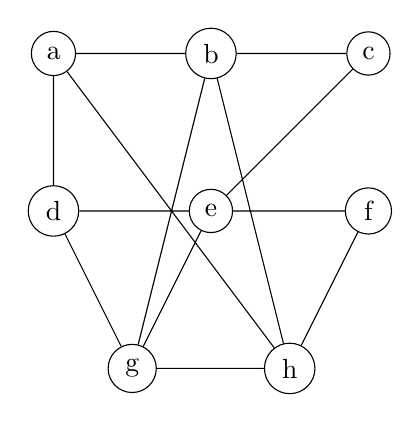
\begin{tikzpicture}
	\node[circle,draw](a) at (0,2) {a};
	\node[circle,draw](b) at (2,2) {b};
	\node[circle,draw](c) at (4,2) {c};
	\node[circle,draw](d) at (0,0) {d};
	\node[circle,draw](e) at (2,0) {e};
	\node[circle,draw](f) at (4,0) {f};
	\node[circle,draw](g) at (1,-2) {g};
	\node[circle,draw](h) at (3,-2) {h};

	\draw (a) -- (b) -- (c) -- (e) -- (d) -- (g) -- (h) -- (f) -- (e) -- (d) -- (a) -- (h) -- (b) -- (g) -- (e);
\end{tikzpicture}
\\
\\
1. Contract \( \left\{ a,d \right\}  \) \\

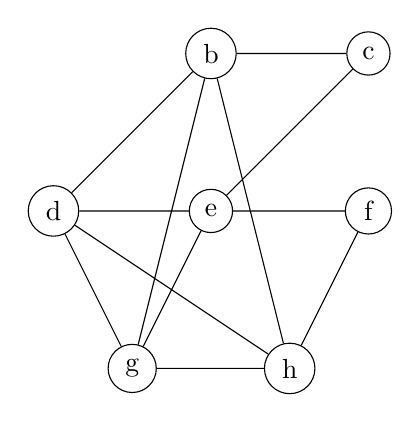
\begin{tikzpicture}
	\node[circle,draw](b) at (2,2) {b};
	\node[circle,draw](c) at (4,2) {c};
	\node[circle,draw](d) at (0,0) {d};
	\node[circle,draw](e) at (2,0) {e};
	\node[circle,draw](f) at (4,0) {f};
	\node[circle,draw](g) at (1,-2) {g};
	\node[circle,draw](h) at (3,-2) {h};

	\draw (d) -- (b) -- (c) -- (e) -- (d) -- (g) -- (h) -- (f) -- (e) -- (d) -- (h) -- (b) -- (g) -- (e);
\end{tikzpicture}
\\
\\
2. Contract \( \left\{ c,e \right\}  \) \\

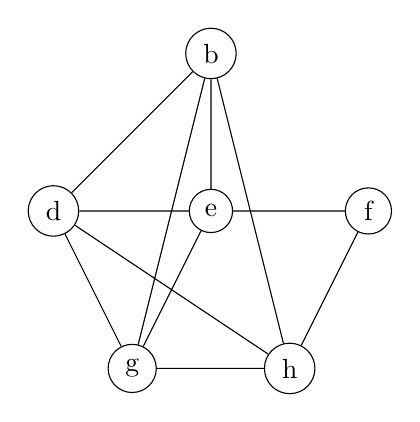
\begin{tikzpicture}
	\node[circle,draw](b) at (2,2) {b};
	\node[circle,draw](d) at (0,0) {d};
	\node[circle,draw](e) at (2,0) {e};
	\node[circle,draw](f) at (4,0) {f};
	\node[circle,draw](g) at (1,-2) {g};
	\node[circle,draw](h) at (3,-2) {h};

	\draw (d) -- (b) -- (e) -- (d) -- (g) -- (h) -- (f) -- (e) -- (d) -- (h) -- (b) -- (g) -- (e);
\end{tikzpicture}
\newpage
3. Contract \( \left\{ f,e \right\}  \) \\

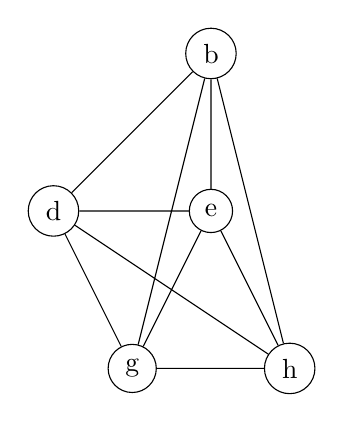
\begin{tikzpicture}
	\node[circle,draw](b) at (2,2) {b};
	\node[circle,draw](d) at (0,0) {d};
	\node[circle,draw](e) at (2,0) {e};
	\node[circle,draw](g) at (1,-2) {g};
	\node[circle,draw](h) at (3,-2) {h};

	\draw (d) -- (b) -- (e) -- (d) -- (g) -- (h) -- (e) -- (d) -- (h) -- (b) -- (g) -- (e);
\end{tikzpicture}

When we rearrange the nodes we can clearly see that it's a \( K_{5} \) graph. Thus \( G \) is not planar.\\
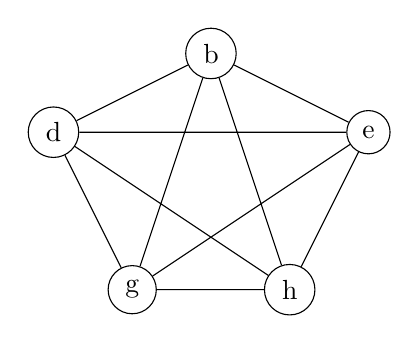
\begin{tikzpicture}
	\node[circle,draw](b) at (2,2) {b};
	\node[circle,draw](d) at (0,1) {d};
	\node[circle,draw](e) at (4,1) {e};
	\node[circle,draw](g) at (1,-1) {g};
	\node[circle,draw](h) at (3,-1) {h};

	\draw (d) -- (b) -- (e) -- (d) -- (g) -- (h) -- (e) -- (d) -- (h) -- (b) -- (g) -- (e);
\end{tikzpicture}
\section*{Exercise \homeworkNumber.2}

\begin{enumerate}[(a)]
	\item
	\item
\end{enumerate}



\section*{Exercise \homeworkNumber.3}

\begin{enumerate}[(a)]
	\item
	\item
\end{enumerate}



\section*{Exercise \homeworkNumber.4}

\begin{enumerate}[(a)]
	\item
	\item
\end{enumerate}



\end{document}
